\let\negmedspace\undefined
\let\negthickspace\undefined
\documentclass[journal,12pt,onecolumn]{IEEEtran}
\usepackage{cite}
\usepackage{amsmath,amssymb,amsfonts,amsthm}
\usepackage{algorithmic}
\usepackage{graphicx}
\graphicspath{{./figs/}}
\usepackage{textcomp}
\usepackage{xcolor}
\usepackage{txfonts}
\usepackage{listings}
\usepackage{enumitem}
\usepackage{mathtools}
\usepackage{gensymb}
\usepackage{comment}
\usepackage{caption}
\usepackage[breaklinks=true]{hyperref}
\usepackage{tkz-euclide} 
\usepackage{listings}
\usepackage{gvv}                                        
%\def\inputGnumericTable{}                                 
\usepackage[latin1]{inputenc}     
\usepackage{xparse}
\usepackage{color}                                            
\usepackage{array}                                            
\usepackage{longtable}                                       
\usepackage{calc}                                             
\usepackage{multirow}
\usepackage{multicol}
\usepackage{hhline}                                           
\usepackage{ifthen}                                           
\usepackage{lscape}
\usepackage{tabularx}
\usepackage{array}
\usepackage{float}
\newtheorem{theorem}{Theorem}[section]
\newtheorem{problem}{Problem}
\newtheorem{proposition}{Proposition}[section]
\newtheorem{lemma}{Lemma}[section]
\newtheorem{corollary}[theorem]{Corollary}
\newtheorem{example}{Example}[section]
\newtheorem{definition}[problem]{Definition}
\newcommand{\BEQA}{\begin{eqnarray}}
\newcommand{\EEQA}{\end{eqnarray}}
\newcommand{\define}{\stackrel{\triangle}{=}}
\theoremstyle{remark}
\newtheorem{rem}{Remark}

\begin{document}
\title{
ASSIGNMENT 1: GATE 2008 \\
    PH : PHYSICS }
\author{AI25BTECH11035 - Sujal Rajani }
\maketitle
\renewcommand{\thefigure}{\theenumi}
\renewcommand{\thetable}{\theenumi}



\textbf{Read the following instructions carefully}
\begin{enumerate}
        \item This question paper contains \textbf{24} printed pages including pages for rough work. Please check all pages and report discrepancy, if any.

    \item Write your registration number, your name and name of the examination centre at the specified locations on the right half of the ORS.

    \item Using HB pencil, darken the appropriate bubble under each digit of your registration number and the letters corresponding to your paper code.

    \item All the questions in this question paper are of objective type.

    \item Questions must be answered on \textbf{O}bjective \textbf{R}esponce \textbf{S}heet \textbf{(OBC)} by darkening the appropriate bubble (marked A, B, C, D) using HB pencil against the question number on the left hand side of the ORS. \textbf{Each question has only one correct answer.} In case you wish to change an answer, erase the old answer completely. More than one answer bubbled against a question will be treated as a wrong answer.

    \item Questions 1 through 20 are 1-mark questions and questions 21 through 85 are 2-mark questions.

    \item Questions 71 through 73 is one set of common data questions, questions 74 and 75 is another pair of common data questions. The question pairs (76, 77), (78, 79), (80, 81), (82, 83) and (84, 85) are questions with linked answers. The answer to the second question of the above pairs will depend on the answer to the first question of the pair. If the first question in the linked pair is wrongly answered or is un-attempted, then the answer to the second question in the pair will not be evaluated.

    \item Un-attempted questions will carry zero marks.
    \item \textbf{NEGATIVE MARKING:} For Q.1 to Q.20, \textit{0.25} mark will be deducted for each wrong answer. For Q.21 to Q.75, \textit{0.5} mark will be deducted for each wrong answer. For the pairs of questions with linked answers, there will be negative marks only for wrong answer to the first question, i.e. for Q.76, Q.78, Q.80, Q.82 and Q.84, \textit{0.5} mark will be deducted for each wrong answer. There is no negative marking for Q.77, Q.79, Q.81, Q.83 and Q.85.

    \item Calculator \textbf{without data connectivity} is allowed in the examination hall.

    \item Charts, graph sheets and tables are NOT allowed in the examination hall.

    \item Rough work can be done on the question paper itself. Additional blank pages are given at the end of the question paper for rough work.
\end{enumerate}

\newpage

\begin{enumerate}
    \item For arbitrary matrices \textit{E,F,G} and \textit{H} , if \textit{EF-FE}=0 then \textit{Trace(EFGH)} is equal to
    \hfill{\brak{\text{GATE PH 2008}}}
    \begin{multicols}{2}
    \begin{enumerate}
        \item \textit{Trace(HGFE)}
         \item \textit{Trace(E).Trace(F).Trace(G).Trace(H)}
        \item \textit{Trace(GFEH)}
        \item \textit{Trace(EGHF)}
    \end{enumerate}
    \end{multicols}
    \item An unitary matrix$\myvec{
a e^{i\alpha} & b \\
c e^{i\beta} & d}
$is given, where \(a, b, c, d, \alpha, \beta\) are real. The inverse of the matrix is
\hfill{\brak{\text{GATE PH 2008}}}
\begin{multicols}{2}
    \begin{enumerate}
    
\item
$\myvec{
a e^{i\alpha} & -c e^{i\beta} \\
b & d}
$

\item 
$\myvec{
a e^{i\alpha} & c e^{i\beta} \\
b & d
}$

\item
$\myvec{
a e^{-i\alpha} & b \\
c e^{-i\beta} & d
}$

\item
$\myvec{
a e^{-i\alpha} & c e^{-i\beta} \\
b & d}
$

 \end{enumerate}
    \end{multicols}
    \item The curl of a vector field $\overrightarrow{F}$ is $2\hat{x}$. Identify the appropriate vector field $\overrightarrow{F}$ from the choices given below.
    \hfill{\brak{\text{GATE PH 2008}}}
\begin{multicols}{2}
    \begin{enumerate}
\item $\overrightarrow{F} = 2z\hat{x} + 3z\hat{y} + 5y\hat{z}$

\item  $\overrightarrow{F} = 3z\hat{y} + 5y\hat{z}$

\item  $\overrightarrow{F} = 3x\hat{y} + 5y\hat{z}$

\item $\overrightarrow{F} = 2\hat{x} + 5y\hat{z}$
\end{enumerate}
    \end{multicols}
    \item A rigid body is rotating about its centre of mass, fixed at the origin, with an angular velocity $\vec{\omega}$ and angular acceleration $\vec{\alpha}$. If the torque acting on it is $\vec{\tau}$ and its angular momentum is $\vec{L}$, the rate of change of its kinetic energy is
    \hfill{\brak{\text{GATE PH 2008}}}
\begin{multicols}{4}
    \begin{enumerate}

\item  $\frac{1}{2} \ \vec{\tau} \cdot \vec{\omega} $ 

\item $ \frac{1}{2} \ \vec{L} \cdot \vec{\omega} $

\item $\frac{1}{2} \ (\vec{\tau} \cdot \vec{\omega} + \vec{L} \cdot \vec{\alpha}) $
\item $ \frac{1}{2} \ \vec{L} \cdot \vec{\alpha}$
\end{enumerate}
    \end{multicols}
\item A cylinder of mass $M$ and radius $R$ is rolling down without slipping on an inclined plane of angle of inclination $\theta$. The number of generalized coordinates required to describe the motion of this system is
\hfill{\brak{\text{GATE PH 2008}}}
\begin{multicols}{4}
    \begin{enumerate}

\item  1
\item  2
\item  4 
\item  6
\end{enumerate}
    \end{multicols}
\item A parallel plate capacitor is being discharged. What is the direction of the energy flow in terms of the Poynting vector in the space between the plates?

\begin{figure}[H]
    \centering
    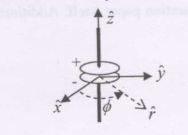
\includegraphics[width = 0.2\columnwidth]{fig/Q.6.png}
    \caption*{}
    \label{fig:Q.6}
\end{figure}
\hfill{\brak{\text{GATE PH 2008}}}
\begin{multicols}{2}
    \begin{enumerate}
\item Along the wire in the positive z axis 
\item Radially inward ($-\hat{r}$ )
\item Radially outward ($-\hat{r}$ )
\item Circumferential  $(\phi)$
\end{enumerate}
    \end{multicols}
\item Unpolarized light falls from air to a planar air-glass interface (refractive index of glass is 1.5) and the reflected light is observed to be plane polarized. The polarization vector and the angle of incidence $\theta_i$ are
\hfill{\brak{\text{GATE PH 2008}}}
    \begin{enumerate}
        \item perpendicular to the plane of incidence and $\theta_i = 42^\circ$
        \item parallel to the plane of incidence and $\theta_i = 56^\circ$
        \item perpendicular to the plane of incidence and $\theta_i = 56^\circ$
        \item parallel to the plane of incidence and $\theta_i = 42^\circ$
    \end{enumerate}

\item A finite wave train, of an unspecified nature, propagates along the positive x axis with a constant speed $v$ and without any change of shape. The differential equation among the four listed below, whose solution it must be, is
\hfill{\brak{\text{GATE PH 2008}}}
\begin{multicols}{2}
    \begin{enumerate}
        \item $\sbrak{\frac{\partial^2}{\partial x^2} - \frac{1}{v^2} \frac{\partial^2}{\partial t^2} } \psi(x,t) = 0$
        
        \item $ \sbrak{\nabla^2 - \frac{1}{v^2} \frac{\partial^2}{\partial t^2}}  \psi(\vec{r},t) = 0$
        
        \item $\sbrak{\frac{\hbar^2}{2m} \frac{\partial^2}{\partial x^2} - i\hbar \frac{\partial}{\partial t}} \psi(x,t) = 0$
        
        \item $ \sbrak{\nabla^2 + a \frac{\partial}{\partial t}}  \psi(\vec{r},t) = 0$
    \end{enumerate}
\end{multicols}

\item Let $| \psi_0 \rangle$ denote the ground state of the hydrogen atom. Choose the correct statement from those given below:
\hfill{\brak{\text{GATE PH 2008}}}
\begin{multicols}{2}
    \begin{enumerate}
        \item $\sbrak{ L_x, L_y } | \psi_0 \rangle = 0$
        \item $J^2 | \psi_0\rangle = 0$
        \item $\vec{L} \cdot \vec{S} | \psi_0 \rangle \neq 0$
        \item $[ S_x, S_y ] | \psi_0 \rangle = 0$
    \end{enumerate}
\end{multicols}

\item Thermodynamic variables of a system can be volume $V$, pressure $P$, temperature $T$, number of particles $N$, internal energy $E$ and chemical potential $\mu$, etc. For a system to be specified by Microcanonical (MC), Canonical (CE) and Grand Canonical (GC) ensembles, the parameters required for the respective ensembles are:

\hfill{\brak{\text{GATE PH 2008}}}
\begin{multicols}{2}
    \begin{enumerate}
        \item MC: $(N,V,T)$; CE: $(E,V,N)$; GC: $(V,T,\mu)$
        \item MC: $(E,V,N)$; CE: $(N,V,T)$; GC: $(V,T,\mu)$
        \item MC: $(V,T,\mu)$; CE: $(N,V,T)$; GC: $(E,V,N)$
        \item MC: $(E,V,N)$; CE: $(V,T,\mu)$; GC: $(N,V,T)$
    \end{enumerate}
\end{multicols}

\item The pressure versus temperature diagram of a given system at certain low temperature range is found to be parallel to the temperature axis in the liquid-to-solid transition region. The change in the specific volume remains constant in this region. The conclusion one can get from the above is

\hfill{\brak{\text{GATE PH 2008}}}
    \begin{enumerate}
        \item the entropy of solid is zero in this temperature region.
        \item the entropy increases when the system goes from liquid to solid phase in this temperature region.
        \item the entropy decreases when the system transforms from liquid to solid phase in this region of temperature.
        \item the change in entropy is zero in the liquid-to-solid transition region.
    \end{enumerate}


\item The radial wave function of the electrons in the state of $n=1$ and $l=0$ in a hydrogen atom is $ R_{10} = \frac{2}{a_0^{3/2}} \exp( -\frac{r}{a_0} )$,where $a_0$ is the Bohr radius. The most probable value of $r$ for an electron is 

\hfill{\brak{\text{GATE PH 2008}}}
\begin{multicols}{4}
    \begin{enumerate}
        \item $a_0$
        \item $2a_0$
        \item $4a_0$
        \item $8a_0$
     \end{enumerate}
\end{multicols}
\item The last two terms of the electronic configuration of manganese (Mn) atom is $3d^5 4s^2$. The term factor of Mn$^{4+}$ ion is
\hfill{\brak{\text{GATE PH 2008}}}
\begin{multicols}{4}
    \begin{enumerate} 
        \item $^4D_{1/2}$
        \item $^4F_{3/2}$
        \item $^3F_{9/2}$
        \item $^3D_{7/2}$
    \end{enumerate}
\end{multicols}

\item The coherence length of laser light is 

\hfill{\brak{\text{GATE PH 2008}}}
    \begin{enumerate}
        \item directly proportional to the length of the active lasing medium.
        \item directly proportional to the width of the spectral line.
        \item inversely proportional to the width of the spectral line.
        \item inversely proportional to the length of the active lasing medium.
    \end{enumerate}

\newpage
\item Metallic monovalent sodium crystallizes in body centered cubic structure. If the length of the unit cell is $4 \times 10^{-8}$ cm, the concentration of conduction electrons in metallic sodium is 

\hfill{\brak{\text{GATE PH 2008}}}
\begin{multicols}{4}
    \begin{enumerate}
        \item $6.022 \times 10^{23} \ \text{cm}^{-3}$
        \item $3.125 \times 10^{22} \ \text{cm}^{-3}$
        \item $2.562 \times 10^{21} \ \text{cm}^{-3}$
        \item $1.250 \times 10^{20} \ \text{cm}^{-3}$
    \end{enumerate}
\end{multicols}


\item The plot of inverse magnetic susceptibility $1/\chi$ versus temperature $T$ of an antiferromagnetic sample corresponds to

\hfill{\brak{\text{GATE PH 2008}}}
\begin{figure}[H]
    \centering
    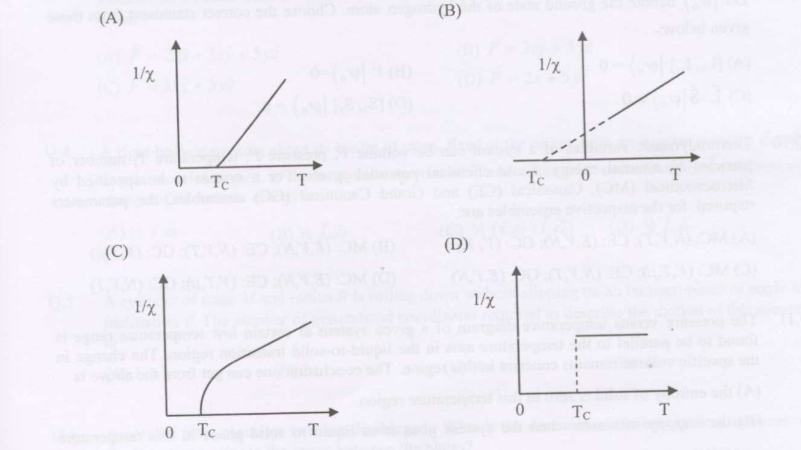
\includegraphics[width = 0.6\columnwidth]{fig/Q.16.png}
    \caption*{}
    \label{fig:Q,16}
\end{figure}
\item According to the quark model, the $K^+$ meson is composed of the following quarks:

\hfill{\brak{\text{GATE PH  2008}}}
\begin{multicols}{4}
    \begin{enumerate}
        \item u u d
        \item u $\bar{c}$
        \item u $\bar{s}$
        \item s $\bar{u}$
    \end{enumerate}
\end{multicols}

\item An O$^{16}$ nucleus is spherical and has a charge radius $R$ and a volume $V \equiv \frac{4}{3} \pi R^3$.  
According to the empirical observations of the charge radii, the volume of the $_{54}$Xe$^{128}$ nucleus, assumed to be spherical, is

\hfill{\brak{\text{GATE PH 2008}}}
\begin{multicols}{4}
    \begin{enumerate}
        \item $8V$
        \item $2V$
        \item $6.75V$
        \item $1.89V$
    \end{enumerate}
\end{multicols}
\item A common emitter transistor amplifier circuit is operated under a fixed bias. In this circuit, the operating point

\hfill{\brak{\text{GATE PH 2008}}}
    \begin{enumerate}
        \item remains fixed with an increase in temperature.
        \item moves towards cut-off region with an increase in temperature.
        \item moves towards the saturation region with a decrease in temperature.
        \item moves towards the saturation region with an increase in temperature.
    \end{enumerate}


\item Under normal operating conditions, the gate terminal of an \textit{n}-channel junction field effect transistor (JFET) and an \textit{n}-channel metal oxide semiconductor field effect transistor (MOSFET) are

\hfill{\brak{\text{GATE PH 2008}}}
    \begin{enumerate}
        \item both biased with positive potentials.
        \item both biased with negative potentials.
        \item biased with positive and negative potentials, respectively.
        \item biased with negative and positive potentials, respectively.
    \end{enumerate}

\item The eigenvalues of the matrix $
 \myvec{
\cos\theta & -\sin\theta \\ \sin\theta & \cos\theta 
}$ are

\hfill{\brak{\text{GATE PH 2008}}}
\begin{multicols}{2}
    \begin{enumerate}
        \item $\frac{1}{2}(\sqrt{3} \pm i) \text{ when } \theta = 45^\circ$
        \item $\frac{1}{2}(\sqrt{3} \pm i) \text{ when } \theta = 30^\circ$
        \item $\pm 1 \text{ since the matrix is unitary}$
        \item $\frac{1}{\sqrt{2}} (1 \pm i) \text{ when } \theta = 30^\circ$
    \end{enumerate}
\end{multicols}

\item If the Fourier transform $F[\delta(x-a)] = \exp(-i 2\pi \nu a)$, then $F^{-1}(\cos 2\pi a \nu)$ will correspond to

\hfill{\brak{\text{GATE PH 2008}}}
\begin{multicols}{2}
    \begin{enumerate}
        \item $\delta(x-a) - \delta(x+a)$
        \item a constant
        \item $\frac{1}{2}[\delta(x-a) + i\delta(x+a)]$
        \item $\frac{1}{2}[\delta(x-a) + \delta(x+a)]$
    \end{enumerate}
\end{multicols}

\item If $I = \oint_C dz \, \mathrm{Ln}(z)$, where $C$ is the unit circle taken anticlockwise and $\mathrm{Ln}(z)$ is the principal branch of the Logarithm function, which one of the following is correct?

\hfill{\brak{\text{GATE PH 2008}}}
\begin{multicols}{2}
    \begin{enumerate}
        \item $I = 0$ by residue theorem.
        \item $I$ is not defined since $\mathrm{Ln}(z)$ has a branch cut.
        \item $I \neq 0$
        \item $\oint_C dz \, \mathrm{Ln}(z^2) = 2I$
    \end{enumerate}
\end{multicols} 
\item The value of $ \int_{-i}^{i} \pi(z+1) \, dz$ is

\hfill{\brak{\text{GATE PH 2008}}}
\begin{multicols}{4}
    \begin{enumerate}
        \item 0
        \item $2\pi i$
        \item $-2\pi i$
        \item $(-1 + 2i)\pi$
    \end{enumerate}
\end{multicols}
\item Consider the Bessel equation ( $\nu = 0$ ),$\frac{d^2 y}{dz^2} + \frac{1}{z}\frac{dy}{dz} + y$ = 0.Which one of the following statements is correct?
\hfill{\brak{\text{GATE PH 2008}}}
    \begin{enumerate}
        \item Equation has regular singular points at $z=0$ and $z=\infty$.
        \item Equation has 2 linearly independent solutions that are entire.
        \item Equation has an entire solution and a second linearly independent solution singular at $z=0$.
        \item Limit $z\to\infty$, taken along $x$ axis, exists for both the linearly independent solutions.
    \end{enumerate}


\item Under a certain rotation of coordinate axes, a rank-1 tensor $v_a$ ($a=1,2,3$) transforms according to the orthogonal transformation defined by the relations$ v'_1 = \frac{1}{\sqrt{2}}(v_1 + v_2), v'_2 =\frac{1}{\sqrt{2}}(-v_1 + v_2) ;v'_3 = v_3.$'
Under the same rotation a rank-2 tensor $T_{a,b}$ would transform such that
\hfill{\brak{\text{GATE PH 2008}}}
\begin{multicols}{2}
    \begin{enumerate}
        \item $T'_{1,1} = T_{1,1}  T_{1,2}$
        \item $T'_{1,1} = T_{1,1}$
        \item $T'_{1,1} = T_{1,1} + 2T_{2,2} - T_{2,1}$
        \item $T'_{1,1} = \tfrac{1}{2}(T_{1,1} + T_{2,2} + T_{1,2} + T_{2,1})$
    \end{enumerate}
\end{multicols}

\item The Lagrangian of a system is given by $  L = \tfrac{1}{2}\dot q^{2} + q\dot q - \tfrac{1}{2} q^{2} $.It describes the motion of
\hfill{\brak{\text{GATE PH 2008}}}
\begin{multicols}{2}
    \begin{enumerate}
        \item a harmonic oscillator.
        \item a damped harmonic oscillator.
        \item an anharmonic oscillator.
        \item a system with unbounded motion.
    \end{enumerate}
\end{multicols}

\item The moment of inertia tensor of a rigid body is given by
$I = [\myvec{
8 & 0 & -4 \\
0 & 4 & 0 \\
-4 & 0 & 8}
$. The magnitude of the moment of inertia about an axis $\hat{n} = \bigl(\tfrac{1}{2},\,\tfrac{\sqrt{3}}{2},\,0\bigr)$ is
\hfill{\brak{\text{GATE PH 2008}}}
\begin{multicols}{4}
    \begin{enumerate}
        \item 6
        \item 5
        \item 2
        \item 8/3
    \end{enumerate}
\end{multicols}

\item A hoop of radius $R$ is pivoted at a point on the circumference. The period of small oscillations in the plane of the hoop is  
\hfill{\brak{\text{GATE PH 2008}}}
\begin{multicols}{4}
\begin{enumerate}
    \item $2\pi \sqrt{\frac{2R}{g}}$
    \item $2\pi \sqrt{\frac{R}{4g}}$
    \item $2\pi \sqrt{\frac{R}{g}}$
    \item $2\pi \sqrt{\frac{9R}{7g}}$
\end{enumerate}
\end{multicols}
\item A mass $m$ is constrained to move on a horizontal frictionless surface. It is set in circular motion with radius $r_{0}$ and angular speed $\omega_{0}$ by an applied force $\overrightarrow{}{F}$ communicated through an inextensible thread that passes through a hole on the surface as shown in the figure. This force is then suddenly doubled. The magnitude of the radial velocity of the mass
\begin{figure}[h!]
    
    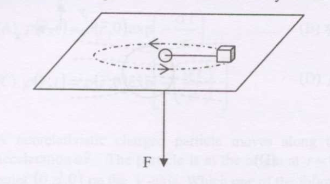
\includegraphics[width=0.5\linewidth]{fig/Q.30.png}
    
    \label{fig:placeholder}
\end{figure}
\hfill{\brak{\text{GATE PH 2008}}}
\begin{enumerate}
    \item increases till the mass falls into the hole.
    \item decreases till the mass falls into the hole.
    \item remains constant.
    \item becomes zero at a radius $r_{1}$ where $0 < r_{1} < r_{0}$.
\end{enumerate}

\item For a simple harmonic oscillator the Lagrangian is given by $L = \tfrac{1}{2} \dot{q}^2 - \tfrac{1}{2} q^2$ If $A(p,q) = \tfrac{p + i q}{\sqrt{2}}$ and $H(p,q)$ is the Hamiltonian of the system, the Poisson bracket $\{ A(p,q), H(p,q) \}$ is given by 
\hfill{\brak{\text{GATE PH 2008}}}
\begin{enumerate}
    \item $i A(p,q)$
    \item $A^{*}(p,q)$
    \item $-i A^{*}(p,q)$
    \item $-i A(p,q)$
\end{enumerate}

\item A plane electromagnetic wave is given by $E_{0}  \hat{x} + e^{i \delta} \hat{y}  \exp \{ i(k z - \omega t) \}$At a given location, the number of times $\vec{E}$ vanishes in one second is
\hfill{\brak{\text{GATE PH 2008}}}
\begin{enumerate}
    \item An integer near $\frac{\omega}{\pi}$ when $\delta = n\pi$ and zero when $\delta \neq n\pi$, $n$ is integer
    \item An integer near $\frac{\omega}{\pi}$ and is independent of $\delta$
    \item An integer near $\frac{\omega}{2\pi}$ when $\delta = n\pi$ and zero when $\delta \neq n\pi$, $n$ is integer
    \item An integer near $\frac{\omega}{2\pi}$ and is independent of $\delta$
\end{enumerate}


\item A dielectric sphere is placed in a uniform electric field directed along the positive $y$-axis. Which one of the following represents the correct equipotential surfaces?
\begin{figure}[H]
    \centering
    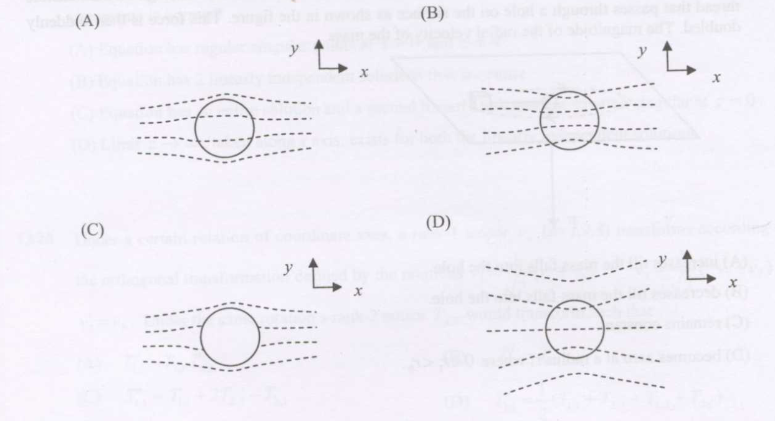
\includegraphics[width = 0.6\columnwidth]{fig/Q.33.png}
    \caption*{}
    \label{fig:Q.33}
\end{figure}
\hfill{\brak{\text{GATE PH 2008}}}
\item A rod of length $L$ with uniform charge density $\lambda$ per unit length is in the $xy$-plane and rotating about the $z$-axis passing through one of its edge with an angular velocity $\boldsymbol{\omega}$ as shown in the figure below. $(\hat{r},\hat{\phi},\hat{z})$ refer to the unit vectors at $Q$, $\vec{A}$ is the vector potential at a distance $d$ from the origin $O$ along $z$-axis for $d >> L$ and $\vec{J}$ is the current density due to the motion of the rod. Which one of the following statements is correct?
\begin{figure}[H]
    \centering
    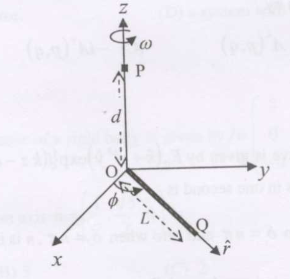
\includegraphics[width = 0.2\columnwidth]{fig/Q.34.png}
    \caption*{}
    \label{fig:Q.34}
\end{figure}
\hfill{\brak{\text{GATE PH 2008}}}
\begin{multicols}{2}
\begin{enumerate}
    \item  $\vec{J}$ along $\hat{r}$; $\vec{A}$ along $\hat{z}$; $|\vec{A}|\propto \dfrac{1}{d}$.
    \item  $\vec{J}$ along $\hat{\phi}$; $\vec{A}$ along $\hat{\phi}$; $|\vec{A}|\propto \dfrac{1}{d^2}$.
    \item  $\vec{J}$ along $\hat{\phi}$; $\vec{A}$ along $\hat{\phi}$; $|\vec{A}|\propto \dfrac{1}{d^2}$.
    \item  $\vec{J}$ along $\hat{\phi}$; $\vec{A}$ along $\hat{\phi}$; $|\vec{A}|\propto \dfrac{1}{d}$.
\end{enumerate}
\end{multicols}
\item A circular disc of radius $a$ on the $xy$ plane has a surface charge density $\sigma = \frac{\sigma_0\, r \cos\theta}{a}$.The electric dipole moment of this charge distribution is
\hfill{\brak{\text{GATE PH 2008}}}
\begin{multicols}{4}
\begin{enumerate}
    \item $\dfrac{\sigma_0 \pi a^4}{4}\,\hat{x}$
    \item $\dfrac{\sigma_0 \pi a^3}{4}\,\hat{x}$
    \item $-\dfrac{\sigma_0 \pi a^3}{4}\,\hat{x}$
    \item $-\dfrac{\sigma_0 \pi a^4}{4}\,\hat{x}$
\end{enumerate}
\end{multicols}
\item At time $t=0$, a charge distribution $\rho(\vec{r},0)$ exists within an ideal homogeneous conductor of permittivity $\varepsilon$ and conductivity $\sigma$. At a later time $\rho(\vec{r},t)$ is given by
\hfill{\brak{\text{GATE PH  2008}}}
\begin{multicols}{2}
\begin{enumerate}
    \item $\rho(\vec{r},t)=\rho(\vec{r},0)\exp\biggl(-\dfrac{\sigma t}{\varepsilon}\biggr)$
    \item $\rho(\vec{r},t)=\dfrac{\rho(\vec{r},0)}{1+\bigl({\sigma t}/{\varepsilon}\bigr)^2}$
    \item $\rho(\vec{r},t)=\rho(\vec{r},0)\exp\biggl[-\biggl(\dfrac{\sigma t}{\varepsilon}\biggr)^2\biggr]$
    \item $\rho(\vec{r},t)=\rho(\vec{r},0)\,\dfrac{\varepsilon}{\sigma t}\sin\!\biggl(\dfrac{\sigma t}{\varepsilon}\biggr)$
\end{enumerate}
\end{multicols}

\item A nonrelativistic charged particle moves along the positive $x$-axis with a constant positive acceleration $a\hat{x}$. The particle is at the origin at $t=0$. Radiation is observed at $t=0$ at a distant point $(0,d,0)$ on the $y$-axis. Which one of the following statements is correct?
\hfill{\brak{\text{GATE PH 2008}}}
\begin{enumerate}
    \item The radiation is unpolarized.
    \item The radiation is plane polarized with polarization parallel to the $x$-axis.
    \item The radiation is plane polarized with polarization parallel to the $xy$ plane along a line inclined to the $x$-axis.
    \item The radiation is elliptically polarized.
\end{enumerate}


\item For a physical system, two observables $O_1$ and $O_2$ are known to be compatible. Choose the correct implication from amongst those given below:
\hfill{\brak{\text{GATE IN 2008}}}
\begin{enumerate}
    \item Every eigenstate of $O_1$ must necessarily be an eigenstate of $O_2$.
    \item Every non-degenerate eigenstate of $O_1$ must necessarily be an eigenstate of $O_2$.
    \item When an observation of $O_1$ is carried out on an arbitrary state $|\Psi\rangle$ of the physical system, a subsequent observation of $O_2$ leads to an unambiguous result.
    \item Observation of $O_1$ and $O_2$, carried out on an arbitrary state $|\Psi\rangle$ of the physical system, lead to identical results irrespective of the order in which the observations are made.
\end{enumerate}
\item An exact measurement of the position of a simple harmonic oscillator (SHO) is made with the result $x = x_0$.  [The SHO has energy levels $E_n$ ($n=0,1,2,\dots$) and associated normalized wave-functions $\psi_n$.]  Subsequently, an exact measurement of energy $E$ is made.  Using the general notation $\Pr(E = E')$ denoting the probability that a result $E'$ is obtained for this measurement, the following statements are written.  Which one of the following statements is correct?
\hfill{\brak{\text{GATE PH 2008}}}
\begin{multicols}{2}
\begin{enumerate}
    \item $\Pr(E = E_0) = 0$
    \item $\Pr(E = E_n) = 1$ for some value of $n$.
    \item $\Pr(E = E_n) \propto \psi_n(x)$
    \item $\Pr(E > E'') > 0$ for any $E''$.
\end{enumerate}
\end{multicols}

\item Consider the combined system of proton and electron in the hydrogen atom in its (electronic) ground state.  Let $I$ denote the quantum number associated with the total angular momentum and let $<M>$ denote the magnitude of the expectation value of the net magnetic moment in the state.  Which of the following pairs represents a possible state of the system ($\mu_B$ is Bohr magneton)?
\hfill{\brak{\text{GATE PH 2008}}}
\begin{multicols}{2}
\begin{enumerate}
    \item $I = 0,<M> = 0$
    \item $I = {1}/{2},<M>= 1\mu_B$
    \item $I = 1,<M>\approx 1\,\mu_B$
    \item $I = 0,<M> \approx 2\,\mu_B$
\end{enumerate}
\end{multicols}
\item A particle is placed in a one dimensional box of size $L$ along the $x$-axis ($0<x<L$). Which of the following is true?
\hfill{\brak{\text{GATE PH 2008}}}
\begin{enumerate}
    \item In the ground state, the probability of finding the particle in the interval $(L/4,\,3L/4)$ is half.
    \item In the first excited state, the probability of finding the particle in the interval $(L/4,\,3L/4)$ is half. This also holds for states with $n=4,6,8,\dots$.
    \item For an arbitrary state $|\Psi\rangle$, the probability of finding the particle in the left half of the well is half.
    \item In the ground state, the particle has a definite momentum.
\end{enumerate}


\item An inelastic ball of mass $m$ has been thrown vertically upwards from the ground at $z=0$. The initial kinetic energy of the ball is $E$. The phase trajectory of the ball after successive bouncing on the ground is
\hfill{\brak{\text{GATE PH 2008}}}
\begin{figure}[H]
    \centering
    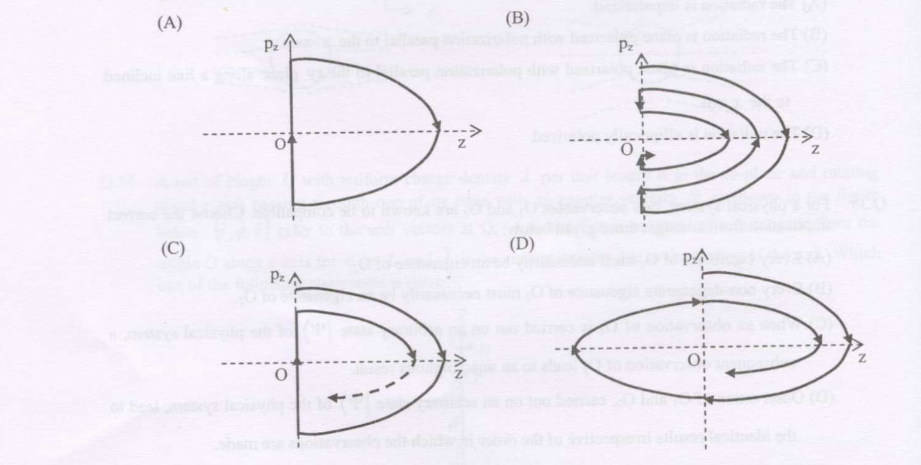
\includegraphics[width = 0.6\columnwidth]{fig/Q42..png}
    \caption*{}
    \label{fig:Q42}
\end{figure}


\item A system containing $N$ non-interacting localized particles of spin $1/2$ and magnetic moment $\mu$ each is kept in a constant external magnetic field $B$ and in thermal equilibrium at temperature $T$. The magnetization of the system is
\hfill{\brak{\text{GATE PH 2008}}}
\begin{multicols}{2}
\begin{enumerate}
    \item $N\mu\coth\biggl(\dfrac{\mu B}{k_B T}\biggr)$
    \item $N\mu\tanh\biggl(\dfrac{\mu B}{k_B T}\biggr)$
    \item $N\mu\sinh\biggl(\dfrac{\mu B}{k_B T}\biggr)$
    \item $N\mu\cosh\biggl(\dfrac{\mu B}{k_B T}\biggr)$
\end{enumerate}
\end{multicols}
\item Two identical particles have to be distributed among three energy levels. Let $r_B,r_F$ and $r_C$ represent the ratios of probability of finding two particles to that of finding one particle in a given energy state. The subscripts \textit{B, F and C} correspond to whether the particles are bosons, fermions and classical particles, respectively. Then $r_B : r_F : r_C$ is equal to
\hfill{\brak{\text{GATE PH 2008}}}
\begin{multicols}{4}
\begin{enumerate}
    \item $\dfrac{1}{2} : 0 : 1$
    \item $1 : \dfrac{1}{2} : 1$
    \item $1 : \dfrac{1}{2} : \dfrac{1}{2}$
    \item $1 : 0 : \dfrac{1}{2}$
\end{enumerate}
\end{multicols}
\item A photon gas is at thermal equilibrium at temperature $T$. The mean number of photons in an energy state $\varepsilon = \hbar\omega$ is
\hfill{\brak{\text{GATE PH 2008}}}
\begin{multicols}{4}
\begin{enumerate}
    \item $\exp\biggl(\dfrac{\hbar\omega}{k_B T}\biggr)+1$
    \item $\exp\biggl(\dfrac{\hbar\omega}{k_B T}\biggr)-1$
    \item $\biggl(\exp\biggl(\dfrac{\hbar\omega}{k_B T}\biggr)+1\biggr)^{-1}$
    \item $\biggl(\exp\!\biggl(\dfrac{\hbar\omega}{k_B T}\biggr)-1\biggr)^{-1}$
\end{enumerate}
\end{multicols}

\item Consider a system of $N$ atoms of an ideal gas of type $A$ at temperature $T$ and volume $V$. It is kept in diffusive contact with another system of $N$ atoms of another ideal gas of type $B$ at the same temperature $T$ and volume $V$. Once the combined system reaches equilibrium,
\hfill{\brak{\text{GATE PH 2008}}}
\begin{enumerate}
    \item the total entropy of the final system is the same as the sum of the entropy of the individual system always.
    \item the entropy of mixing is $2N k_B \ln 2$.
    \item the entropy of the final system is less than that of sum of the initial entropies of the two gases.
    \item the entropy of mixing is non-zero when the atoms $A$ and $B$ are of the same type.
\end{enumerate}


\item Consider a system of two non-interacting classical particles which can occupy any of the three energy levels with energy values $E=0,\varepsilon$ and $2\varepsilon$ having degeneracies $g(E)=1,2$ and $4$ respectively. The mean energy of the system is
\hfill{\brak{\text{GATE PH 2008}}}
\begin{multicols}{2}
\begin{enumerate}
    \item $\varepsilon\biggl(\frac{4\exp(-\varepsilon/k_B T)+8\exp(-2\varepsilon/k_B T)}{1+2\exp(-\varepsilon/k_B T)+4\exp(-2\varepsilon/k_B T)}\biggr)$
    \item $ \varepsilon\biggl(\frac{2\exp(-\varepsilon/k_B T)+8\exp(-2\varepsilon/k_B T)}{1+2\exp(-\varepsilon/k_B T)+4\exp(-2\varepsilon/k_B T)}\biggr)$
    \item $ \varepsilon\biggl(\frac{2\exp(-\varepsilon/k_B T)+4\exp(-2\varepsilon/k_B T)}{1+2\exp(-\varepsilon/k_B T)+4\exp(-2\varepsilon/k_B T)}\biggr)^{2}$
    \item $ \varepsilon\biggl(\frac{\exp(-\varepsilon/k_B T)+2\exp(-2\varepsilon/k_B T)}{1+\exp(-\varepsilon/k_B T)+\exp(-2\varepsilon/k_B T)}\biggr)   $
\end{enumerate}
\end{multicols}

\item Three consecutive absorption lines at $64.275\ \text{cm}^{-1},\ 77.130\ \text{cm}^{-1}$ and $89.985\ \text{cm}^{-1}$ have been observed in a microwave spectrum for a linear rigid diatomic molecule. The moments of inertia $I_A$ and $I_B$ are ($I_A$ is with respect to the bond axis passing through the centre of mass and $I_B$ is with respect to an axis passing through the centre of mass and perpendicular to bond axis)
\hfill{\brak{\text{GATE PH 2008}}}
\begin{multicols}{2}
\begin{enumerate}
    \item both equal to $\dfrac{\hbar^2}{12.855\,h c} \mathrm{gmcm^2}$
    \item zero and $\dfrac{\hbar^2}{12.855\,h c}\ \mathrm{gmcm^2}$
    \item both equal to $\dfrac{\hbar^2}{6.427\,h c}\ \mathrm{gmcm^2}$
    \item zero and $\dfrac{\hbar^2}{6.427\,h c}\ \mathrm{gmcm^2}$
\end{enumerate}
\end{multicols}

\item A pure rotational Raman spectrum of a linear diatomic molecule is recorded using electromagnetic radiation of frequency $\nu_e$. The frequency of two consecutive Stokes lines are
\hfill{\brak{\text{GATE PH 2008}}}
\begin{multicols}{2}
\begin{enumerate}
    \item $\nu_e - 10B, \nu_e - 14B$
    \item $\nu_e - 2B, \nu_e - 4B$
    \item $\nu_e + 10B, \nu_e + 14B$
    \item $\nu_e + 2B,\nu_e + 4B$
\end{enumerate}
\end{multicols}

  \item Which one of the following statement is \textbf{INCORRECT} in vibrational spectroscopy with anharmonicity?
  \hfill{\brak{\text{GATE PH 2008}}}
\begin{multicols}{2}
\begin{enumerate}
    \item The selection rule for vibrational spectroscopy is$\Delta\nu=\pm1,\pm2,\dots$
    \item Anharmonicity leads to multiple absorption lines.
    \item The intensities of hot band lines are stronger than the fundamental absorption.
    \item The frequencies of hot band lines are smaller than the fundamental absorption.
\end{enumerate}
\end{multicols}

\item The molecular spectra of two linear molecules O-C-O and O-C-S are recorded in the microwave region. Which one of the following statement is correct?
\hfill{\brak{\text{GATE PH 2008}}}
\begin{multicols}{2}
\begin{enumerate}
    \item Both the molecules would show absorption lines.
    \item Both the molecules would not show absorption lines.
    \item O-C-O would show absorption lines, but not O-C-S.
    \item O-C-S would show absorption lines, but not O-C-O.
\end{enumerate}
\end{multicols}

\item When the refractive index $\mu$ of the active medium changes by $\Delta\mu$ in a laser resonator of length $L$, the change in the spectral spacing between the longitudinal modes of the laser is(c is the speed of light in free space)
\hfill{\brak{\text{GATE PH 2008}}}
\begin{multicols}{4}
\begin{enumerate}
    \item $\dfrac{c}{2(\mu+\Delta\mu)L}$
    \item $\dfrac{c}{2\Delta\mu\,L}$
    \item $\dfrac{c}{2L}\,\dfrac{\Delta\mu}{\mu(\mu+\Delta\mu)}$
    \item zero.
\end{enumerate}
\end{multicols}

\item The primitive translation vectors of the body centered cubic lattice are $\vec{a}=\dfrac{a}{2}(\hat{x}+\hat{y}-\hat{z})$, $\vec{b}=\dfrac{a}{2}(-\hat{x}+\hat{y}+\hat{z})$ and $\vec{c}=\dfrac{a}{2}(\hat{x}-\hat{y}+\hat{z})$. The primitive translation vectors $\vec{A},\vec{B}$ and $\vec{C}$ of the reciprocal lattice are
\hfill{\brak{\text{GATE PH 2008}}}
\begin{enumerate}
    \item $\vec{A}=\dfrac{2\pi}{a}(\hat{x}-\hat{y})$;\quad $\vec{B}=\dfrac{2\pi}{a}(\hat{y}+\hat{z})$;\quad $\vec{C}=\dfrac{2\pi}{a}(\hat{x}+\hat{z})$
    \item $\vec{A}=\dfrac{2\pi}{a}(\hat{x}+\hat{y})$;\quad $\vec{B}=\dfrac{2\pi}{a}(\hat{y}-\hat{z})$;\quad $\vec{C}=\dfrac{2\pi}{a}(\hat{x}+\hat{z})$
    \item $\Vec{A}=\dfrac{2\pi}{a}(\hat{x}+\hat{y})$;\quad $\vec{B}=\dfrac{2\pi}{a}(\hat{y}+\hat{z})$;\quad $\vec{C}=\dfrac{2\pi}{a}(\hat{x}-\hat{z})$
    \item $\vec{A}=\dfrac{2\pi}{a}(\hat{x}+\hat{y})$;\quad $\vec{B}=\dfrac{2\pi}{a}(\hat{y}+\hat{z})$;\quad $\vec{C}=\dfrac{2\pi}{a}(\hat{x}+\hat{z})$
\end{enumerate}

\item The structure factor of a single cell of identical atoms of form factor $f$ is given by $S_{hkl}=f\sum_j \exp\!\bigl(-i2\pi(x_s h + y_s k + z_s l)\bigr)$,where $(x_j ,y_j ,z_j)$ is the coordinate of an atom, and $hkl$ are the Miller indices. Which one of the following statements is correct for the diffraction peaks of body centered cubic (BCC) and face centered cubic (FCC) lattices?
\hfill{\brak{\text{GATE PH 2008}}}
\begin{multicols}{2}
\begin{enumerate}
    \item BCC : (200); (110); (222) \\
          FCC : (111); (311); (400)
    \item BCC : (210); (110); (222) \\
          FCC : (111); (311); (400)
    \item BCC : (200); (110); (222) \\
          FCC : (111); (211); (400)
    \item BCC : (200); (210); (222) \\
          FCC : (111); (211); (400)
\end{enumerate}
\end{multicols}
\item The lattice specific heat $C$ of a crystalline solid can be obtained using the Dulong-Petit model, Einstein model and Debye model. At low temperature $\hbar\omega >> k_B T$, which one of the following statements is true ($a$ and $A$ are constants)
\hfill{\brak{\text{GATE PH 2008}}}
\begin{enumerate}
    \item Dulong-Petit : $C\propto\exp(-a/T)$;Einstein : $C=\text{constant}$; Debye : $C\propto\bigl(\tfrac{T}{A}\bigr)^3$
    \item Dulong-Petit : $C=\text{constant}$; Einstein : $C\propto\bigl(\tfrac{T}{A}\bigr)^3$;Debye : $C\propto\exp(-a/T)$
    \item Dulong-Petit : $C=\text{constant}$;  Einstein : $C\propto\dfrac{e^{-a/T}}{T^2}$; Debye : $C\propto\bigl(\tfrac{T}{A}\bigr)^3$
    \item Dulong-Petit : $C\propto\bigl(\tfrac{T}{A}\bigr)^3$;Einstein : $C\propto\dfrac{e^{-a/T}}{T^2}$;Debye : $C=\text{constant}$
\end{enumerate}


\item A linear diatomic lattice of lattice constant $a$ with masses $M$ and $m$ ($M>m$) are coupled by a force constant $C$. The dispersion relation is given by
\begin{align*}
\omega_{\pm}^2 = C\biggl(\frac{M+m}{Mm}\biggr) \pm \biggl[\,C^2\!\Bigl(\frac{M+m}{Mm}\Bigr)^2 - \frac{4C^2}{Mm}\sin^2\!\frac{ka}{2}\,\biggr]^{1/2}
\end{align*}
then Which one of the following statements is \textbf{INCORRECT}?
\hfill{\brak{\text{GATE PH 2008}}}
\begin{enumerate}
    \item The atoms vibrating in transverse mode correspond to the optical branch.
    \item The maximum frequency of the acoustic branch depends on the mass of the lighter atom $m$.
    \item The dispersion of frequency in the optical branch is smaller than that in the acoustic branch.
    \item No normal modes exist in the acoustic branch for any frequency greater than the maximum frequency at $k=\pi/a$.
\end{enumerate}

\item The kinetic energy of a free electron at a corner of the first Brillouin zone of a two dimensional square lattice is larger than that of an electron at the mid-point of a side of the zone by a factor $b$. The value of $b$ is
\hfill{\brak{\text{GATE PH 2008}}}
\begin{multicols}{4}
\begin{enumerate}
    \item b = $\sqrt{2}$
    \item b = 2
    \item b = 4
    \item b = 8
\end{enumerate}
\end{multicols}

\item An intrinsic semiconductor with mass of a hole $m_h$, and mass of an electron $m_e$, is at a finite temperature $T$. If the top of the valence band energy is $E_v$ and the bottom of the conduction band energy is $E_c$, the Fermi energy of the semiconductor is
\hfill{\brak{\text{GATE PH 2008}}}
\begin{multicols}{2}
\begin{enumerate}
    \item $E_F = \biggl(\dfrac{E_v+E_c}{2}\biggr) - \dfrac{3}{4} k_B T \ln\biggl(\dfrac{m_h}{m_e}\biggr)$
    \item $E_F = \biggl(\dfrac{k_B T}{2}\biggr) + \dfrac{3}{4}(E_v+E_c)\ln\biggl(\dfrac{m_h}{m_e}\biggr)$
    \item $E_F = \biggl(\dfrac{E_v+E_c}{2}\biggr) + \dfrac{3}{4} k_B T \ln\biggl(\dfrac{m_h}{m_e}\biggr)$
    \item $E_F = \biggl(\dfrac{k_B T}{2}\biggr) - \dfrac{3}{4}(E_v+E_c)\ln\biggl(\dfrac{m_h}{m_e}\biggr)$
\end{enumerate}
\end{multicols}

\item Choose the correct statement from the following:
\hfill{\brak{\text{GATE PH 2008}}}
\begin{enumerate}
    \item The reaction $K^+ K^- \to p\bar{p}$ can proceed irrespective of the kinetic energies of $K^+$ and $K^-$.
    \item The reaction $K^+ K^- \to p\bar{p}$ is forbidden by baryon number conservation.
    \item The reaction $K^+ K^- \to 2\gamma$ is forbidden by strangeness conservation.
    \item The decay $K^0 \to \pi^+ \pi^-$ proceeds via weak interactions.
\end{enumerate}

\item The following gives a list of pairs containing (i) a nucleus (ii) one of its properties. Find the pair which is \underline{\textbf{INAPPROPRIATE}}
\hfill{\brak{\text{GATE PH 2008}}}
\begin{enumerate}
    \item (i) ${}^{20}\mathrm{Ne}$ nucleus; \quad (ii) stable nucleus.
    \item (i) A spheroidal nucleus; \quad (ii) an electric quadrupole moment.
    \item (i) ${}^{16}\mathrm{O}$ nucleus; \quad (ii) nuclear spin $J=1/2$.
    \item (i) ${}^{238}\mathrm{U}$ nucleus; \quad (ii) Binding energy $=1785\ \mathrm{MeV}$ (approximately).
\end{enumerate}


\item The four possible configurations of neutrons in the ground state of  $_4\mathrm{Be}^9$ nucleus, according to the shell model, and the associated nuclear spin are listed below. Choose the correct one:
\hfill{\brak{\text{GATE PH 2008}}}
\begin{multicols}{2}
\begin{enumerate}
    \item $(1s_{1/2})^2(1p_{3/2})^2$; \quad $J=3/2$
    \item $(1s_{1/2})^2(1p_{1/2})^2(1p_{3/2})^2$; \quad $J=3/2$
    \item $(1s_{1/2})^2(1p_{3/2})^4$; \quad $J=1/2$
    \item $(1s_{1/2})^2(1p_{3/2})^2(1p_{1/2})^1$; \quad $J=1/2$
\end{enumerate}
\end{multicols}

\item The mass difference between the pair of mirror nuclei $_{6}\mathrm{C}^{11}$ and $_{5}\mathrm{B}^{11}$ is given to be $\Delta{MeV}/c^2$. According to the semi-empirical mass formula, the mass difference between the pair of mirror nuclei $_{9}\mathrm{F}^{17}$ and $_{8}\mathrm{O}^{17}$ will approximately be (rest mass of proton $m_p=938.27{MeV}/c^2$ and rest mass of neutron $m_n=939.57\ \mathrm{MeV}/c^2$)
\hfill{\brak{\text{GATE PH 2008}}}
\begin{multicols}{2}
\begin{enumerate}
    \item $1.39\Delta{MeV}/c^2$
    \item $(1.39\Delta + 0.5){MeV}/c^2$
    \item $0.864\Delta{MeV}/c^2$
    \item $(1.6\Delta + 0.78){MeV}/c^2$
\end{enumerate}
\end{multicols}

\item A heavy nucleus is found to contain more neutrons than protons.  This fact is related to which one of the following statements?
\hfill{\brak{\text{GATE PH 2008}}}
\begin{enumerate}
    \item The nuclear force between neutrons is stronger than that between protons.
    \item The nuclear force between protons is of a shorter range than those between neutrons, so that a smaller number of protons are held together by the nuclear force.
    \item Protons are unstable, so their number in a nucleus diminishes.
    \item It costs more energy to add a proton to a (heavy) nucleus than a neutron because of the Coulomb repulsion between protons.
\end{enumerate}


\item A neutral pi meson ($\pi^0$) has a rest-mass of approximately $140\ \mathrm{MeV}/c^2$ and a lifetime of $\tau$ sec. A $\pi^0$ produced in the laboratory is found to decay after $1.25\tau$ sec into two photons. Which of the following sets represents a possible set of energies of the two photons as seen in the laboratory?
\hfill{\brak{\text{GATE PH 2008}}}
\begin{multicols}{2}
\begin{enumerate}
    \item 70MeV and 70MeV                                                \item 35MeV and 100MeV
    \item 75MeV and 100MeV
    \item 25MeV and 150MeV
\end{enumerate}
\end{multicols}

\item An a.c. voltage of $220{V_{rms}}$ is applied to the primary of a $10:1$ step-down transformer. The secondary of the transformer is centre tapped and connected to a full wave rectifier with a load resistance. The d.c. voltage appearing across the load is
\hfill{\brak{\text{GATE PH 2008}}}
\begin{multicols}{4}
\begin{enumerate}
    \item $\dfrac{22}{\pi}$
    \item $\dfrac{31}{\pi}$
    \item $\dfrac{62}{\pi}$
    \item $\dfrac{44}{\pi}$
\end{enumerate}
\end{multicols}

\item Let $I_1$ and $I_2$ represent mesh currents in the loop $abcda$ and $befcb$ respectively. The correct expression describing Kirchhoff's voltage loop law in one of the following loops is
\begin{figure}[H]
    \centering
    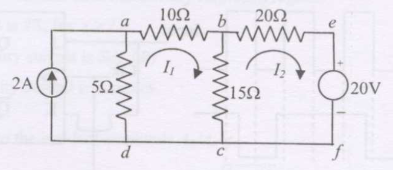
\includegraphics[width = 0.6\columnwidth]{fig/Q.66.png}
    \caption*{}
    \label{fig:Q.66}
\end{figure}
\hfill{\brak{\text{GATE PH 2008}}}
\begin{multicols}{2}
\begin{enumerate}
    \item $30 I_1 - 15 I_2 = 10$
    \item $-15 I_1 + 20 I_2 = -20$
    \item $30 I_1 - 15 I_2 = -10$
    \item $-15 I_1 + 20 I_2 = 20$
\end{enumerate}
\end{multicols}

\item The simplest logic gate circuit corresponding to the Boolean expression $Y = P + \overline{P}Q$ is
\hfill{\brak{\text{GATE PH 2008}}}
\begin{figure}[H]
    \centering
    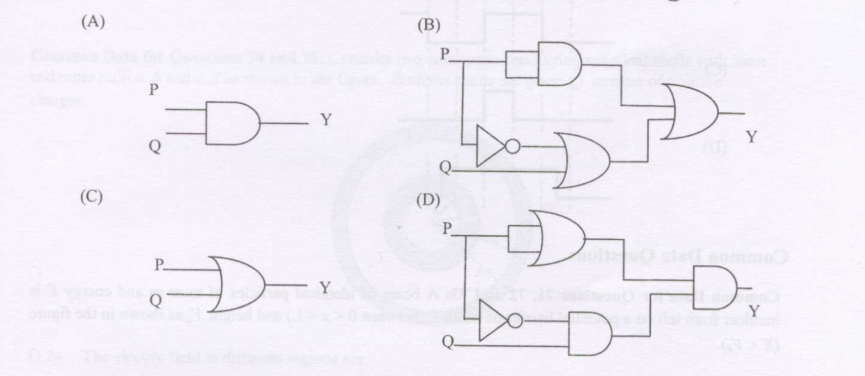
\includegraphics[width = 0.6\columnwidth]{fig/Q.67.png}
    \caption*{}
    \label{fig:Q67}
\end{figure}
\item An analog voltage $V$ is converted into a 2-bit binary number. The minimum number of comparators required and their reference voltages are
\hfill{\brak{\text{GATE PH 2008}}}
\begin{multicols}{2}
\begin{enumerate}
    \item $3, \bigl(\tfrac{V}{4},\tfrac{V}{2},\tfrac{3V}{4}\bigr)$
    \item $3, \bigl(\tfrac{V}{3},\tfrac{2V}{3},V\bigr)$
    \item $4, \bigl(\tfrac{V}{5},\,\tfrac{2V}{5},\,\tfrac{3V}{5},\,\tfrac{4V}{5}\bigr)$
    \item $4,\bigl(\tfrac{V}{4},\tfrac{V}{2},\tfrac{3V}{4},V\bigr)$
\end{enumerate}
\end{multicols}

\item The following circuit (where $R_L \gg R$) performs the operation of
\begin{figure}[H]
    \centering
    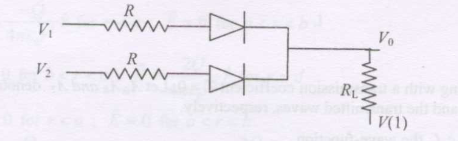
\includegraphics[width = 0.6\columnwidth]{fig/Q.69.png}
    \caption*{}
    \label{fig:Q69}
\end{figure}
\hfill{\brak{\text{GATE PH 2008}}}
\begin{multicols}{2}
\begin{enumerate}
    \item OR gate for a negative logic system
    \item NAND gate for a negative logic system
    \item AND gate for a positive logic system
    \item AND gate for a negative logic system
\end{enumerate}
\end{multicols}
 
\item In the T-type master-slave JK flip-flop shown along with the clock and input waveforms, the $Q_n$ output of the flip-flop was zero initially. Identify the correct output waveform.
\begin{figure}[H]
    \centering
    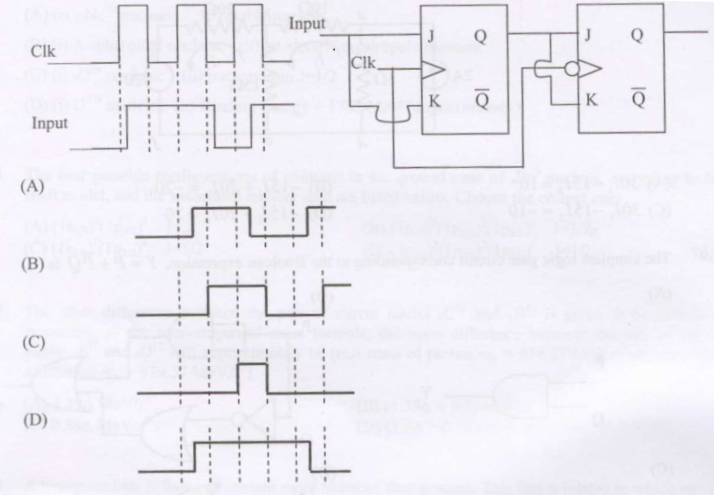
\includegraphics[width = 0.6\columnwidth]{fig/Q.70.png}
    \caption*{}
    \label{fig:Q70}
\end{figure}
\hfill{\brak{\text{GATE PH 2008}}}
\section*{Common Data Question} 
\textbf{Common Data for  Questions 71,72 and 73}: A beam of identical particles of mass m and energy E is incident from left on a potential barrier of width L (between $0<x<L$) and height $v_0$ as shown in the figure (E$<$ $V_0$ ).
\begin{figure}[H]
    \centering
    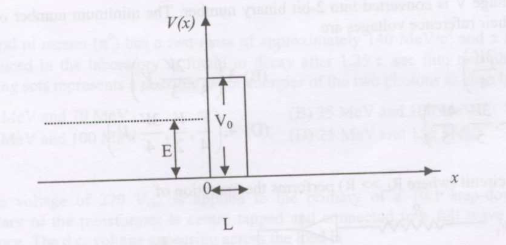
\includegraphics[width = 0.6\columnwidth]{fig/Q71 to Q73.png}
    \caption*{}
    \label{fig:Q71 to Q73}
\end{figure}
 For x$>$L there is tunneling with a transmission coefficient T>0. Let $A_0$,$A_R$ and $A_T$  denote the amplitudes for the incident, reflected and transmitted waves, respectively.

\item Throughout $0<x<L$, the wave-function
\hfill{\brak{\text{GATE PH 2008}}}
\begin{multicols}{2}
\begin{enumerate}
    \item can be chosen to be real.
    \item is exponentially decaying.
    \item is generally complex.
    \item is zero.
\end{enumerate}
\end{multicols}

\item Let the probability current associated with the incident wave be $S_0$. Let $R$ be the reflection coefficient. Then
\hfill{\brak{\text{GATE PH 2008}}}
\begin{enumerate}
    \item the probability current vanishes in the classically forbidden region.
    \item the probability current is $T S_0$ for $x>L$.
    \item for $x<0$, the probability current is $S_0(1+R)$.
    \item for $x>L$, the probability current is complex.
\end{enumerate}


\item The ratio of the reflected to the incident amplitude $A_R/A_0$ is
\hfill{\brak{\text{GATE PH 2008}}}
\begin{multicols}{2}
\begin{enumerate}
    \item $1 - \dfrac{A_T}{A_0}$
    \item $\sqrt{1-T}$ in magnitude
    \item a real negative number
    \item $ \sqrt{\,1 - \biggl|\dfrac{A_T}{A_0}\biggr|^{2}\dfrac{E}{V_0 - E}}$
\end{enumerate}
\end{multicols}
\vspace{0.5mm}
\textbf{Common Data for Questions 74 and 75:} 
Consider two concentric conducting spherical shells with inner and outer radii a, b and c, d as shown in the figure. Both the shells are given Q amount of positive charges.

% Figure placeholder
% \begin{center}
% \includegraphics[width=0.5\textwidth]{figure_name.png}
% \end{center}

\begin{figure}[H]
    \centering
    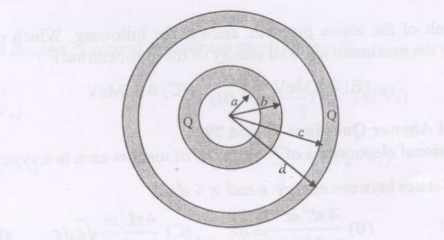
\includegraphics[width = 0.6\columnwidth]{fig/Q74 to Q75.png}
    \caption*{}
    \label{fig:Q74 to Q75}
    \end{figure}
\item The electric field in different regions are
\hfill{\brak{\text{GATE PH 2008}}}
\begin{enumerate}
    \item $\vec{E}=0$ for $r<a$;\quad $\vec{E}=-\dfrac{Q}{4\pi\varepsilon_0 r^2}\hat{r}$ for $a<r<b$ \\
    \quad $\vec{E}=0$ for $b<r<c$;\quad $\vec{E}=\dfrac{Q}{4\pi\varepsilon_0 r^2}\hat{r}$ for $r>d$
    \item $\vec{E}=-\dfrac{Q}{4\pi\varepsilon_0 r^2}\hat{r}$ for $r<a$;\quad $\vec{E}=0$ for $a<r<b$ \\
    \quad $\vec{E}=\dfrac{Q}{4\pi\varepsilon_0 r^2}\hat{r}$ for $b<r<c$;\quad $\vec{E}=\dfrac{Q}{4\pi\varepsilon_0 r^2}\hat{r}$ for $r>d$
    \item $\vec{E}=-\dfrac{Q}{4\pi\varepsilon_0 r^2}\,\hat{r}$ for $r<a$;\quad $\vec{E}=0$ for $a<r<b$ \\
    \quad $\vec{E}=0$ for $b<r<c$;\quad $\vec{E}=\dfrac{2Q}{4\pi\varepsilon_0 r^2}\,\hat{r}$ for $r>d$
    \item $\vec{E}=0$ for $r<a$;\quad $\vec{E}=0$ for $a<r<b$ \\
    \quad $\vec{E}=\dfrac{Q}{4\pi\varepsilon_0 r^2}\hat{r}$ for $b<r<c$;\quad $\vec{E}=\dfrac{2Q}{4\pi\varepsilon_0 r^2}\hat{r}$ for $r>d$
\end{enumerate}


\item In order to have equal surface charge densities on the outer surfaces of both the shells, the following conditions should be satisfied
\hfill{\brak{\text{GATE PH 2008}}}
\begin{multicols}{2}
\begin{enumerate}
    \item $d = 4b$ and $c = 2a$
    \item $d = 2b$ and $c = \sqrt{2}\,a$
    \item $d = \sqrt{2}\,b$ and $c > a$
    \item $d > b$ and $c = \sqrt{2}\,a$
\end{enumerate}
\end{multicols}
\vspace{0.5 mm}
\section* {Linked Answer Questions: Q.76 to Q.85 carry two marks each.}
\vspace{0.5 mm}
\textbf{Statement for Linked Answer Questions 76 and 77:} 
Consider the $\beta$-decay of a free neutron at rest in the laboratory.
\vspace{0.25 mm}
        \item Which of the following configurations of the decay products correspond to the largest energy of the anti-neutrino? (rest mass of electron $m_e$=$0.51MeV/{c^2}$,rest mass of proton $m_p$=$938.27MeV/{c^2}$ and rest mass of electron $m_n$=$939.57MeV/{c^2}$

\begin{enumerate}
    \item In the laboratory, proton is produced at rest.
    \item In the laboratory, momenta of proton, electron and the anti-neutrino all have the same magnitude.
    \item In the laboratory, proton and electron fly-off with (nearly) equal and opposite momenta.
    \item In the laboratory, electron is produced at rest.
\end{enumerate}


        \item Using the result of the above problem, which of the    following  represents approximately the maximum allowed energy of the anti-neutrino {$\bar\nu$}?
        \hfill{\brak{\text{GATE PH 2008}}}
\begin{multicols}{4}
\begin{enumerate}
    \item 1.3{MeV}
    \item 0.8{MeV}
    \item 0.5{MeV}
    \item 2.0{MeV}
\end{enumerate}
\end{multicols}
\vspace{0.5 mm}
\textbf{Statement for Linked Answer Questions 78 and 79:} 
Consider a two dimensional electron gas of \(N\) electrons of mass \(m\) each in a system of size $L \times L$.
\vspace{0.25 mm}

\item The density of states between energy $\varepsilon$ and $\varepsilon + d\varepsilon$ is
\hfill{\brak{\text{GATE PH 2008}}}
\begin{multicols}{4}
\begin{enumerate}
    \item $\dfrac{4\pi L^2 m}{h^2}d\varepsilon$
    \item $\dfrac{4\pi L^2 m}{h^2}\dfrac{1}{\sqrt{\varepsilon}}d\varepsilon$
    \item $\dfrac{4\pi L^2 m}{h^2}\sqrt{\varepsilon}d\varepsilon$
    \item $\dfrac{4\pi L^2 m}{h^2}\varepsilon d\varepsilon$
\end{enumerate}
\end{multicols}

\item The ground state energy $E_0$ of the system in terms of the Fermi energy $E_F$ and the number of electrons $N$ is given by
\hfill{\brak{\text{GATE PH 2008}}}
\begin{multicols}{4}
\begin{enumerate}
    \item $\tfrac{1}{3} N E_F$
    \item $\tfrac{1}{2} N E_F$
    \item $\tfrac{2}{3} N E_F$
    \item $\tfrac{3}{5} N E_F$
\end{enumerate}
\end{multicols}
\vspace{0.5 mm}
\textbf{Statement for Linked Answer Questions 80 and 81:} 
The rate of a clock in a spaceship ``Suryashakti'' is observed from earth to be ${3}/{5}$ of the rate of the clocks on earth.
\vspace{0.25 mm}

\item The speed of the spaceship "Suryashakti" relative to earth is
\hfill{\brak{\text{GATE PH 2008}}}
\begin{multicols}{4}
\begin{enumerate}
    \item $\dfrac{4}{5}c$
    \item $\dfrac{3}{5}c$
    \item $\dfrac{9}{10}c$
    \item $\dfrac{2}{5}c$
\end{enumerate}
\end{multicols}

\item The rate of a clock in a spaceship "Aakashganga" is observed from earth to be 5/13 of the rate of the clocks on earth. If both Aakashganga and Suryashakti are moving in the same direction relative to someone on earth, then the speed of Aakashganga relative to Suryashakti is
\hfill{\brak{\text{GATE PH 2008}}}
\begin{multicols}{4}
\begin{enumerate}
    \item $\dfrac{12}{13}c$
    \item $\dfrac{4}{5}c$
    \item $\dfrac{8}{17}c$
    \item $\dfrac{5}{6}c$
\end{enumerate}
\end{multicols}
\begin{figure}[H]
    \centering
    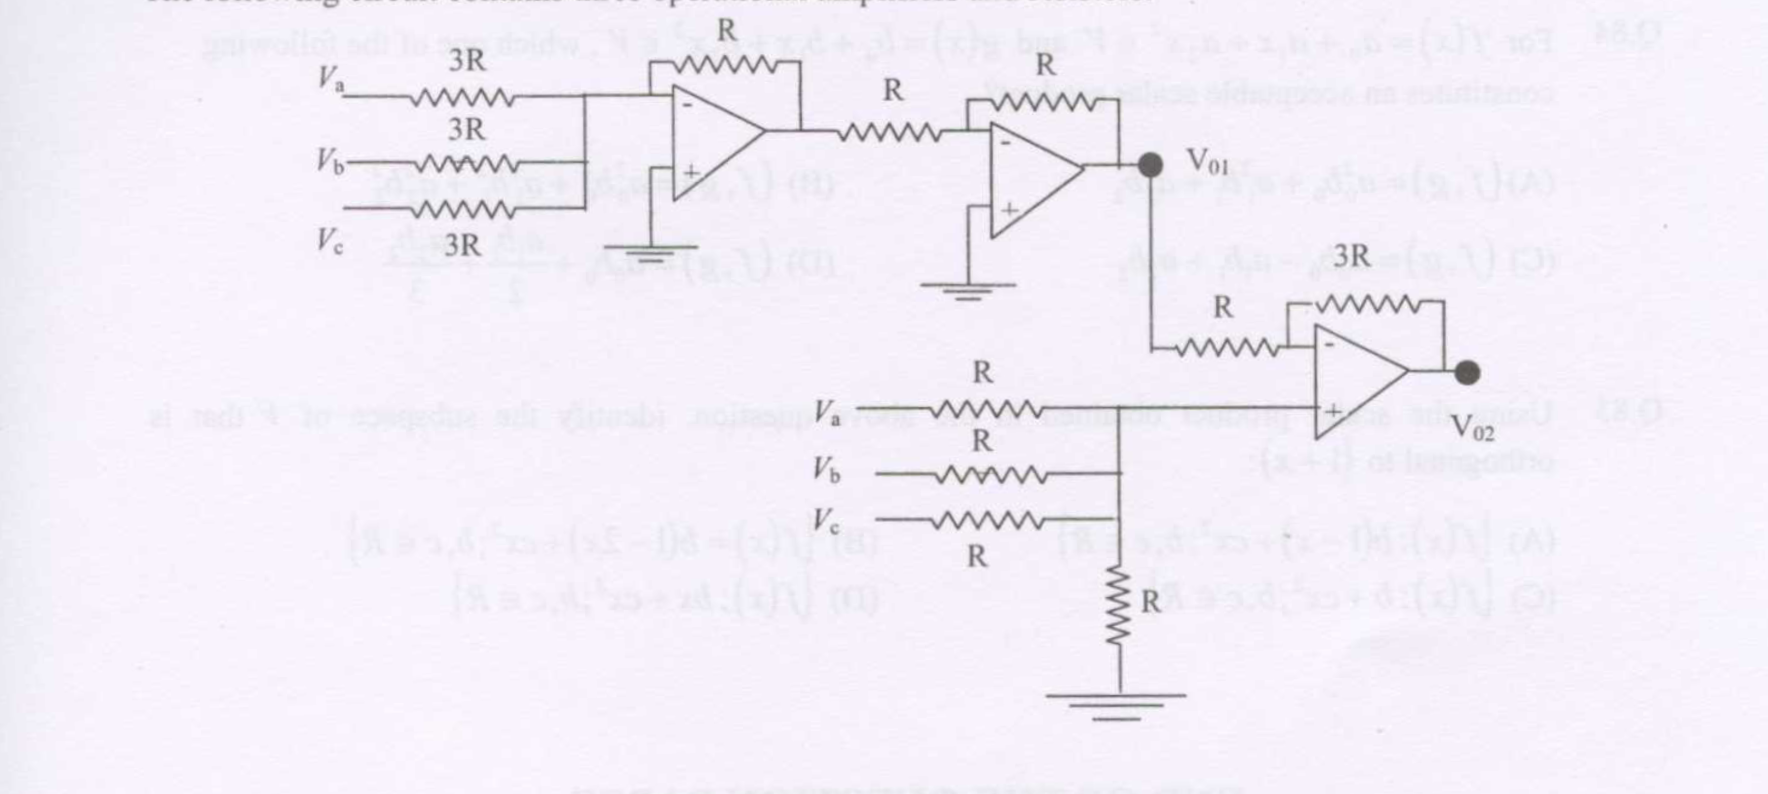
\includegraphics[width = 0.6\columnwidth]{fig/Q82 to Q83.png}
    \caption*{}
    \label{fig:Q82 to Q83}
    \end{figure}
\vspace{0.5 mm}
\textbf{Statement for Linked Answer Questions 82 and 83:} 
The following circuit contains three operational amplifiers and resistors.
\vspace{0.25 mm}

\item The output voltage at the end of second operational amplifier $V_{o1}$ is
\hfill{\brak{\text{GATE PH 2008}}}
\begin{multicols}{2}
\begin{enumerate}
    \item $V_{o1}=3(V_a+V_b+V_c)$
    \item $V_{o1}=-\tfrac{1}{3}(V_a+V_b+V_c)$
    \item $V_{o1}=\tfrac{1}{3}(V_a+V_b+V_c)$
    \item $V_{o1}=\tfrac{4}{3}(V_a+V_b+V_c)$
\end{enumerate}
\end{multicols}

\item The output $V_{o2}$ (at the end of third op amp) of the above circuit is
\hfill{\brak{\text{GATE PH 2008}}}
\begin{multicols}{2}
\begin{enumerate}
    \item $V_{o2}=2(V_a+V_b+V_c)$
    \item $V_{o2}=3(V_a+V_b+V_c)$
    \item $V_{o2}=-\tfrac{1}{2}(V_a+V_b+V_c)$
    \item Zero
\end{enumerate}
\end{multicols}

\vspace{0.5 mm}
\textbf{Statement for Linked Answer Questions 84 and 85:} 
The set $V$ of all polynomials of a real variable x of degree two or less and with real coefficients, constitutes a real linear vector space $V \{\equiv \{ c_{0} + c_{1}x + c_{2}x^{2} : c_{0}, c_{1}, c_{2}\} \in \mathbb{R}$ 

\item For $f(x)=a_0 + a_1x + a_2 x^2 \in\mathbb{V}$ and $g(x) = b_0 + b_1 x + b_2  x^2 \in\mathbb{V} $, which one of the following constitutes an acceptable scalar product?
\hfill{\brak{\text{GATE PH 2008}}}
\begin{multicols}{2}
\begin{enumerate}
    \item $(f,g)=a_0^2 b_0 + a_1^2 b_1 + a_2^2 b_2$
    \item $(f,g)=a_0^2 b_0^2 + a_1^2 b_1^2 + a_2^2 b_2^2$
    \item $(f,g)=a_0 b_0 - a_1 b_1 + a_2 b_2$
    \item $(f,g)=a_0 b_0 + \dfrac{a_1 b_1}{2} + \dfrac{a_2 b_2}{3}$
\end{enumerate}
\end{multicols}

\item Using the scalar product obtained in the above question, identify the subspace of $V$ that is orthogonal to $(1 + x)$:
\hfill{\brak{\text{GATE PH 2008}}}
\begin{multicols}{2}
\begin{enumerate}
    \item $\{f(x): b(1-x)+c x^2 ; b,c\in\mathbb{R}\}$
    \item $\{f(x): b(1-2x)+c x^2 ; b,c\in\mathbb{R}\}$
    \item $\{f(x):b + c x^2 ; b,c\in\mathbb{R}\}$
    \item $\{f(x): b x + c x^2 ; b,c\in\mathbb{R}\}$
\end{enumerate}
\end{multicols}
\vspace{2mm}
\begin{center}
    \section*{END OF THE QUESTION PAPER}
\end{center}
\end{enumerate}

\end{document}